% !TEX TS-program = pdflatex
% !TEX encoding = UTF-8 Unicode

% This is a simple template for a LaTeX document using the "article" class.
% See "book", "report", "letter" for other types of document.

\documentclass[11pt]{article} % use larger type; default would be 10pt

\usepackage[utf8]{inputenc} % set input encoding (not needed with XeLaTeX)

%%% Examples of Article customizations
% These packages are optional, depending whether you want the features they provide.
% See the LaTeX Companion or other references for full information.

%%% PAGE DIMENSIONS
\usepackage{geometry} % to change the page dimensions
\geometry{a4paper} % or letterpaper (US) or a5paper or....
% \geometry{margin=2in} % for example, change the margins to 2 inches all round
% \geometry{landscape} % set up the page for landscape
%   read geometry.pdf for detailed page layout information

\usepackage{graphicx} % support the \includegraphics command and options

% \usepackage[parfill]{parskip} % Activate to begin paragraphs with an empty line rather than an indent

%%% PACKAGES
\usepackage{booktabs} % for much better looking tables
\usepackage{array} % for better arrays (eg matrices) in maths
\usepackage{paralist} % very flexible & customisable lists (eg. enumerate/itemize, etc.)
\usepackage{verbatim} % adds environment for commenting out blocks of text & for better verbatim
\usepackage{subfig} % make it possible to include more than one captioned figure/table in a single float
% These packages are all incorporated in the memoir class to one degree or another...

%%% HEADERS & FOOTERS
\usepackage{fancyhdr} % This should be set AFTER setting up the page geometry
\pagestyle{fancy} % options: empty , plain , fancy
\renewcommand{\headrulewidth}{0pt} % customise the layout...
\lhead{}\chead{}\rhead{}
\lfoot{}\cfoot{\thepage}\rfoot{}

%%% SECTION TITLE APPEARANCE
\usepackage{sectsty}
\allsectionsfont{\sffamily\mdseries\upshape} % (See the fntguide.pdf for font help)
% (This matches ConTeXt defaults)

%%% ToC (table of contents) APPEARANCE
\usepackage[nottoc,notlof,notlot]{tocbibind} % Put the bibliography in the ToC
\usepackage[titles,subfigure]{tocloft} % Alter the style of the Table of Contents
\renewcommand{\cftsecfont}{\rmfamily\mdseries\upshape}
\renewcommand{\cftsecpagefont}{\rmfamily\mdseries\upshape} % No bold!

\renewcommand{\labelitemi}{$\bullet$}
\renewcommand{\labelitemii}{$\cdot$}
\renewcommand{\labelitemiii}{$\diamond$}
\renewcommand{\labelitemiv}{$\ast$}

%%% END Article customizations

%%% The "real" document content comes below...

\title{RASD}
\author{Giorgio Pea, Andrea Sessa}
%\date{} % Activate to display a given date or no date (if empty),
         % otherwise the current date is printed

\begin{document}
\maketitle
\newpage

\tableofcontents

\newpage

\section{Introduction}
  \subsection{Purpose}
      This document represent the Requirement Analysis and Specification Document
    (RASD). The main goal of this document is to completely describe the system
    in terms of functional and non-functional requirements, to show the constraints and the limit
    of the software and simulate the typical use cases that will occur after the
    development. This document is intended to all developer and programmer who
    have to implement the requirements, to system analyst who want to integrate
    other system with this one, and could be used as a contractual basis between
    the customer and the developer.

  \subsection{Scope of the project}
   The aim of this project is to develop MyTaxiService, a web/mobile application that makes easier and quicker taking taxies.
    Thanks to MyTaxiService, anyone can request or book a taxi and get realtime information
    about how long it will take to be picked up or about taxi's current position and code.
    In addition, MyTaxiService provides an efficient way to allocate taxies by dividing the
    city in zones and using a queue based allocation system, in order to reduce the
    waiting time and city's traffic.
  \subsection{Project Perspective}

    \subsection{Goals}
        In this subsection we describe a set of high level goals that MyTaxiService is proposed to achieve.\newline
      \begin{enumerate}
        \item Simplify and speed up the process of taking a taxi
        \begin{itemize}
          \item When a registered user has entered his taxi ride details and clicks or taps
      the "REQUEST TAXI" button, MyTaxiService will find the first
      available taxi that fits for the inserted ride details, and this taxi will
      pick up the user as soon as possible

          \item When a registered user has entered his booking details and clicks or taps
        the "BOOK TAXI" button, MyTaxiService will book a taxi that fits for the
        inserted booking details and for the indicated pick up time
        \end{itemize}
        \item Guarantee an efficient and fair management of taxi queues
        \begin{itemize}
          \item Guarantee a balanced distribution of taxies in the city, in order
      to have always taxies available for different city zones
          \item Guarantee short taxi availability times and short waiting times
         \end{itemize}
      \end{enumerate}
      
        \subsection{Assumptions}
    \begin{enumerate}
        \item MyTaxiService has been commissioned by the city local government.
      Taxi drivers that work in the city can join MyTaxiService via a registration to be
      done in the local government public transport office.
      During this registration process taxi drivers are asked to provide their personal and vehicle data along with their work timetable.
      After that taxi drivers receive a unique code that identifies their taxi cab in relation to MyTaxiService.
      To make MyTaxiService functional, the local government provides each mtaxi with a device similar to a small navigator(MYT), which is used
      to see incoming ride requests or bookings and to signal their acceptance; this device has a built in gps module through which MyTaxiService can
      track their position
    \item The registration of taxies to MyTaxyService is done manually by the local government public transportation
    officiers by inserting records in a db accessed by MyTaxyService, hence in this document that process is
    not modelled
    \item Since MyTaxiService is aware of the work timetable of each mtaxi, mtaxies are considered unavailable
      if and only if they are serving a ride/booking request.  After a mtaxi has finished serving a passenger, its driver has to notify
      MyTaxiService(B) of the event, so MyTaxiService(B) will consider the mtaxi available again.
      Considering that MyTaxiService(B) knows the position of each mtaxi and the destination of each ride, there's no chance a mtaxi driver
      can cheat by not signaling he hasn't completed a ride yet.

    \item A mtaxi might have an accident, if that happens, its driver can report it and therefore
       be considered unavailable

    \item Once a registered user sends a ride request, he or she cannot change any detail of the request nor can
        undo the request(FR)

    \item MyTaxiService(B) is aware of the characteristics of each mtaxies (number of passengers, unique code)

    \item MyTaxiService(B) is aware of all the possible valid location in the city, so a registered user that wants to request a ride or a booking is forced to select one among them.

    \item Mtaxies can accept only ride request/booking within the city borders

    \item Mtaxies can only serve only ride/booking requests forwarded by MyTaxiService(B)

    \item Using gps data from the mtaxies and public traffic data, MyTaxyService(B) can balance the assigment
    of the request so that  .... (RF)
    \end{enumerate}
      
    \subsection{Glossary}

        \subsubsection{Terms disambiguation}
        
        \begin{description}
        
         \item [MyTaxiService(B)] \hfill \\ The back end of MyTaxiService, that is to say, those software components that manage the forwarding of ride / booking requests to the mtaxi drivers, the search of available mtaxies compatible with the received ride/booking requests, and other internal
        tasks not exposed to user or the mtaxi drivers
      \item [Mtaxi] \hfill \\ a taxi whose driver has joined MyTaxyService
      \item [Ride request] \hfill \\ An electronic message sent by a registered user
        to MyTaxiService(B). This electronic message refers to the case in which the registered user wants to be picked up as soon as possible by a mtaxi
      \item [Booking request] \hfill \\ An electronic message sent by a registered user
         to MyTaxiService(B). This electronic message refers to the case in which the registered user wants to be picked up by a mtaxi at a specific time
      \item [Mtaxy booking] \hfill \\ when a registered user wants to be picked up by a mtaxi at a specific time
      \item [MYT] \hfill \\ the device the local government provides to taxi drivers that has registered to MyTaxiService. This
      device integrates a client for MyTaxiService that the is used by the mtaxi driver to see ride/booking requests and zone change orderds, accept
      these requests and report accidents
      \item [A mtaxi is available] \hfill \\ a mtaxi has finished serving a passenger and is ready for a new ride
      \item [Zone] \hfill \\ An area of the city
      \item [Credentials] \hfill \\ A combination of username and password, used by a registered user to access the MyTaxiService application
      \item [Mtaxi ride] \hfill \\ A movement of people, through a taxi cab, from one geographical point to another
      \item [Queue] \hfill \\ A data structure managed with a FIFO policy.
      \item [User] \hfill \\ A person who wants to take a taxi and is not registered to MyTaxiService.
      \item [Registered User] \hfill \\ A person who is not a mtaxy driver, who needs to take a taxi and is registered to MyTaxiService.
      \item [Visitor]\hfill \\ A generic person not registered to MyTaxiService
      \item [Ride/booking request acceptance] \hfill \\ a mtaxi has left in oder to pick up registered user that has requested a ride or that has booked a ride
       \end{description}

      \subsubsection{Acronyms}
      \begin{description}
        \item [RASD:] Requirements Analysis and Specification Document
        \item [FIFO:] First In First Out
       \end{description}

    \subsection{Reference Documents}
       \begin{itemize}
       	\item Specification Document: MyTaxiService-AA2015-2016.pdf
        	\item IEEE Std 830-1998 IEEE Recommended Practice for Software Requirements Specifications.
        	\item IEEE Std 1016 tm -2009 Standard for Information Tecnology-System Design-Software Design Descriptions.
       \end{itemize}
  

\section{Requirements Specification}

    \subsection {Functional Requirements}
    	\begin{enumerate}
    	\item \textbf{[FR1]} A person must not be already registered to MyTaxiService in order perform the registration process
     	\item \textbf{[FR2]} During the registration process, a visitor must choose a username not already used by another user.
      	\item \textbf{[FR3]}A Visitor can only access to the MyTaxiService registration form.
      	\item \textbf{[FR4] }Registered users cannot sign up twice but only once for session.
      	\item \textbf{[FR5] }The login is successful iff the user inserts the correct credentials
      	\item \textbf{[FR6] }The user, after a successful login can submit a taxi request
      	\item \textbf{[FR7] }The user, after a successful login can submit a taxi reservation
      	\item \textbf{[FR8] }The registered users can undo only reservations
      	\item \textbf{[FR9] }The registered users can  undo a reservation only 10 minutes before the inserted
      		picking up time
      	\item \textbf{[FR10]} MyTaxiService has to allow multiple mtaxi bookings by the same registered user
      	\item \textbf{[FR11] }MyTaxiService has not to allow multiple ride requests by the same registered user
      	\item \textbf{[FR12]} MyTaxiService has to be able to force a registered user to chose as locations only valid city's locations
      		(MyTaxiService has to be able to force a registered user to chose among a list of only valid city's locations )
      	\item \textbf{[FR13] } MyTaxiService(B) can accept only ride requests that specify a starting location, an ending location
      		and a number of passengers
      	\item \textbf{[FR14] }MyTaxiService(B) has to be able, using the gps data of the mtaxies and public data about the city's, to understand the
      		traffic situation of the city zone per zone
      	\item \textbf{[FR15] }MyTaxiService(B) has to be able, using the gps data of the mtaxies, to analyse the mtaxies'
      		distribution among the different city's zone and understand if there's the need to change this
      		distribution in relation to the average number of ride /booking requests per city's zone.
      		If there's this need, MyTaxiService(B) has to be able to send change zone order to mtaxies
      	\item \textbf{[FR16] }MyTaxiService(B) has to be able, using the gps data of the mtaxies, to analyse the mtaxies'
      		distribution among the different city's zone and build the queues used to forward ride / booking
      		requests
      	\item \textbf{[FR17] }MyTaxiService(B) has to be able to manage a situation in which a mtaxi does not accept a ride / booking request within a fixed time.
      		In this situation MyTaxiService has to find a new mtaxi to forward the request
      	\item \textbf{[FR18] }MyTaxiDriver has to manage the forwarding of ride / booking requests using a queue based system and
      		a division of the city in zone: foreach city's zone a queue of available mtaxies is associated,
     		MyTaxiDriver(B) forward a ride/booking request to head of the queue that corresponds to the city's
      		zone of the starting location of the ride
      	\item \textbf{[FR19] }Only logged registered users must have access to all the functionalities of MyTaxiService
      	\item \textbf{[FR20] }Visitors have access only to the registration functionality of MyTaxiService
      	\item \textbf{[FR21] }MyTaxiService app and website must have the same functionalities
      	\end{enumerate}


    \subsection {Non Functional Requirements}

    \subsection {Constraints}
    \begin{enumerate}
	\item \textbf{[C1]} A taxi that joins this service has to mount a GPS system
        	\item \textbf{[C2]} The taxies that partecipate to the service can only manage request and reservation from myTaxiService
    \end{enumerate}
    \subsection {Domain Properties}
    \begin{enumerate}
	\item \textbf{[D1]} Time must be included between 00.00 and 23.59.
        	\item \textbf{[D2]} Email address used for registration must be formally correct.
    \end{enumerate}
    \subsection {Jackson-Zave approach}


\section {Scenario and UseCase definition}
  \subsection {Scenario Identification}
  \begin{enumerate}
        \item Funes is a product manager with a very busy schedule. At 11.00 he has a meeting
          with a group of clients to discuss about the features of a new product.
          This meeting is located in a another part of the city.
          For his shifts Funes usually takes taxies, and, in order to speed up this process, he
          started using MyTaxiService.
          Its 10:30 and Funes decides to take a taxi via myTaxiService. He opens the app,
          the app remembers his credentials and logs him in.
          Funes inserts the address of the meeting and of his current location, choses one passenger and taps
          the big request button. MyTaxiService then alerts him that is finding a taxi.
          Near Funes' location, a Taxi has finished serving a passenger, so myTaxiService(B) signals to it
          Funes' request. Assuan, the driver of the Taxi, despite the fact that it's still work time, wants to take a coffee
          and so ignores the request. After 5 mins myTaxiService tries to find a new Taxi
          for Funes: Nabucodonosor's Taxi is available and MyTaxiService forwards Funes' request to it.
          Nabucodonosor receives the request and alerts MyTaxiService that he's going to take care of it.
          myTaxiService alerts Funes that his taxi will arrive in 3 mins.
          The Taxi arrives, and in 10 min Funes reaches the meeting place. MyTaxiService
          signals the behavior of Assuan to his supervisors, and, after a few weeks, Assuan receives a warning and a fine of 200 euro.

        \item It's Monday morning and Bob, an important manager of a very big company, as to attend an important
           conference on Tuesday at 9:00 AM. Unfortunately he has no one
           to take him to the airport on Tuesday morning, also he is very worried to miss his flight tomorrow
           morning due to the lack of available taxi(Tuesday morning is a terrible day!).
           If he will miss the conference, his boss will fire him! Suddenly he remember that the myTaxiService
           application give him the possibility to reserve a taxi ride.
           He pick-up his smartphone, opens the myTaxiService app, enters his credentials and access to the application.
           On the main page he press the 'Reserve' button, a form appear and he enters the time of departure, the point of departure
           and the number of passengers(he himself) then he press the 'Submit' button. The myTaxiService backend receives the request
           and after some calculus notify Bob of the successful registration of its request. Bob is very happy and continues
           its work with a smile on his face.

         \item It's Friday, 11 AM and Ann has been on holiday for three weeks. It's time to go home!
           Ann has booked her return flight for today at 12 AM. Ann has carefully planned the return trip, indeed
           yesterday she made a taxi ride reservation through the myTaxiService web site, but the taxi is in late!
           So she take her smartphone opens the myTaxiService application, enters her credentials and after a successful login
           she presses the 'View Status' button and discovers that her taxi is stuck in a terrible traffic jam.
           "I'll miss my flight!" she thinks, and starts to wait with the heart full of hope.[OK]

        \item Dave, an experienced taxi driver of the city, has received, through myTaxiService, a request for a ride
           from a passenger. "It's not too much far from where i am now", he thinks, "It'll be easy", and notifies
           MyTaxiService that he'll take care of the request. He starts driving toward the passenger's position, but suddenly
           , while he's crossing a very busy crossroad,
           a reckless driver coming from the left crosses at high speed the crossroad and hits with violence
           Dave's taxi cab. Luckily nobody gets hurt, but Dave's taxi cabe has been seriously damaged.
           Dave cannot fulfill the passenger's request so he takes his smartphone, opens the myTaxiService app,
           and taps the "REPORT ACCIDENT" button, he accesses a screen where he inserts the accident details and taps the "SUBMIT" button.
           MyTaxiService(B) receives the Dave's report and after some computations selects and notifies another driver to fulfill the passenger request.
           
          \item Ann, a young female student from Texas, is visiting Italy with his boyfriend Bob.
          It's Friday morning, they are walking on the streets of Milan and they're thinking
          about visiting the Expo on Saturday. Ann proposes to use a taxi to reach Expo's location,
          Bob agrees. Ann is a very cautious person so she thinks its better to book a taxi, for this
          reason she searches on Google "taxi milano book" and discovers MyTaxiService.
          She downloads the app on her Iphone. She opens the app which displays a log in screen with
          a registration button, she taps that button and so access a registration screen she inserts
          her mail address, she choses a password, she confirms that password, she accepts the legal
          terms of the app and taps the confirm button; after that Ann is ready to use the app.
          In order to book a taxi for Saturday for the Expo, Ann accesses the booking section of the app,
          taps the "ADD BOOKING" button and in the add booking screen inserts the Expo's location by selecting the right item in a dropdown menu, inserts the time and location of the picking
          , choses two passengers and taps the big "BOOK TAXI" button, MyTaxiService responds by alerting Ann that her booking
          has been processed successfully. Ann is happy about the fact that everything has proceeded without problems.
          Bob instead is not so happy because he thinks that the Milan's transportation system is perfect
          to reach Expo and its far way cheaper than taking a taxi. Bob and Ann have a brief discussion
          about this and, at the end, Ann agrees with Bob. Given that, Ann tries to undo the booking:
          she opens the app, she logs in, she accesses the booking section and there she sees her booking for Saturday, she taps
          the bin icon to delete the booking, she confirms her intention to do that and everything is done.

         \item It's Thursday, 14:00 and George, a young taxi driver, is driving in the city's center.
           He noticed that many of his colleagues waiting for requests in their cabs.
           Meanwhile MyTaxiService(B), by making some analysis on the taxies' GPS data, realizes that there are to many taxies
           in the city's center in relation with the number of ride requests for that zone. The system also indentifies
           some zones of the city where the concentration of taxies is too low. According to a policy based on some statistical data
           MyTaxiService(B) decides to move 10 taxies, including the George's one, from the city's center to the city's zones mentioned above.
          As a consequence of that, George receives by MyTaxiService a notification that alerts him to move to zone C (one of the city's zones
          with low concentration of taxies). George start driving towards zone C and continues his work.
        \end{enumerate}
        
        
        
  \subsection {Use Case diagram}
  In the following picture is shown an overall perspective of the defined use case and of their relation.
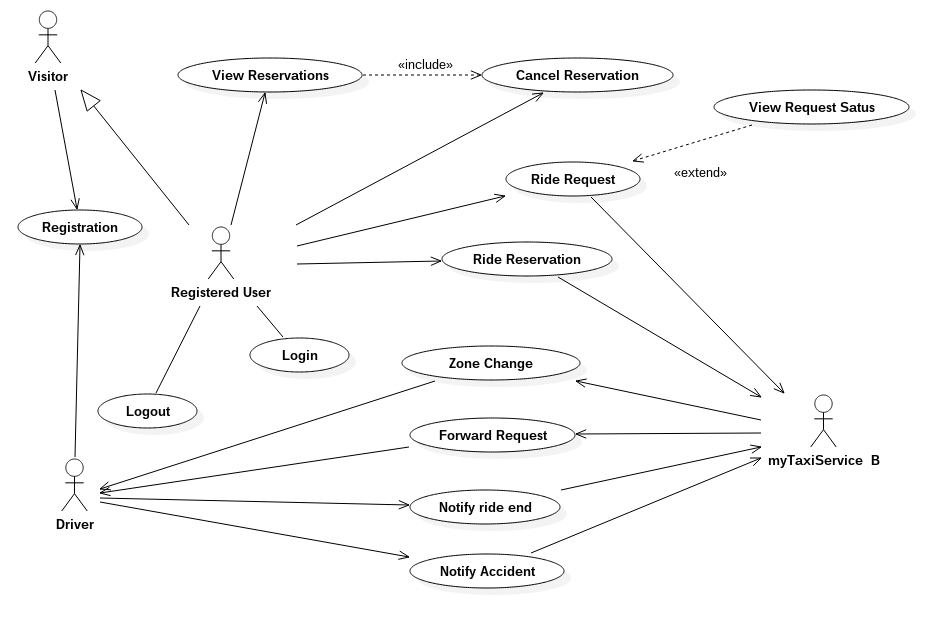
\includegraphics[scale=0.4]{usecase.png}

\subsubsection{Use Case 1}
	A registered user makes a ride request
	\begin{description}
	\item [Use Case name:]Ride request
	\item [Actors:] A registered user, MyTaxiService(B)
       	\item [Pre-cons:] The registered user has logged into MyTaxiService.
        	\item [Post-cons:] MyTaxiService(B) receives the ride request and tries to find an available taxi to fulfill it.
        	\item [Entry Cnd:] A registered user wants to be picked up by a mtaxi as soon as possible in given place.
        	\item [Exit Cnd:] The registered is acknowledge that MyTaxiService(B) has received successfully the ride
        		request
        	\item[Exceptions:]\hfill \\
          		- Connection lost on the smartphone: the registered user is immediately notified of the fact and
          			he can only check the last retrieved status of his ride request
        	\item [Flow of events:]\hfill \\
          		- The registered user taps/clicks the "REQUEST TAXI" button\newline
          		- The registered user is redirected to a screen dedicated to the insertion
          			of the requested ride's details\newline
          		- The registered user fills out a form for the ride request inserting the ride's starting and ending location
          		and the number of passengers and th.\newline
          		- The registered user submits to MyTaxiService(B) the form by clicking/tapping the "CONFIRM REQUEST" button\newline
           \item[Special Requirements:] \hfill \\
          		- The registered user must be acknowledged that MyTaxiService(B) has received successfully the ride request
          		  within 1 min
	\end{description}
	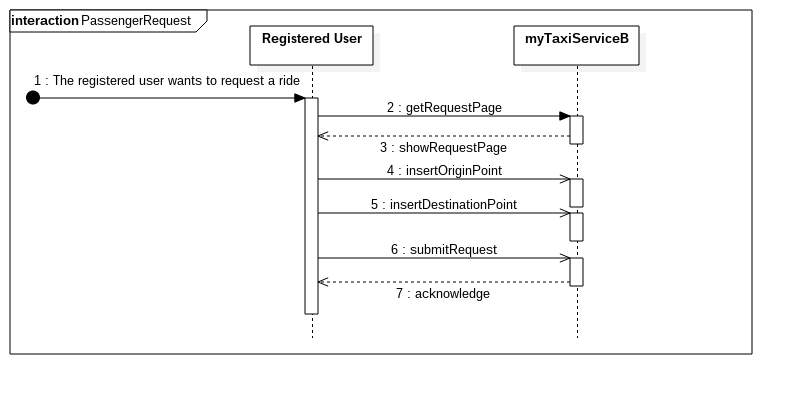
\includegraphics[scale=0.6]{usecase1SD.png}
\subsubsection{Use Case 2}


\end{document}
